\title{ CDA Notes }
\author{Jedediyah Williams}
\date{\today}

\documentclass{article}
\usepackage{mathtools}
\usepackage{amsmath}
\usepackage{graphics}
\usepackage{graphicx}
\usepackage{subfig}
\usepackage{wrapfig}
\usepackage{color,soul}

\begin{document}

What follows contains notes and more detailed derivation and explenation of portions of certain portions of Binh's thesis.  Where appropriate, I'll try to note relevant sections as well as corresponding equation numbers from the thesis.  

\hspace{10cm} - Jed

Newton-Euler equations (2.1) writen in matrix form: \\
\begin{equation}
\mathbf{M}(\mathbf{q},t)\dot{\nu} = \lambda_{vp}(\mathbf{q},\dot{\mathbf{q}},t) + \lambda_{app}(\mathbf{q},t) \tag{2.27}
\end{equation}

Section 2.3.3.3 is straight forward and introduces the complementarity form of the non-penetration constraint.  

Section 2.4.* shows the MCP formulations (linear and nonlinear) both as equations and in matrix form.  

\begin{equation}
0 \leq \mathbf{\lambda}_n^{l+1} \perp \mathbf{W}_n^T \nu^{l+1} + \frac{\Psi_n^l}{h} + \frac{\partial \Psi_n^l}{\partial t} \geq 0 \tag{3.2}
\end{equation}

Section 3.4 introduces Prox functions.  

Section 3.5.1 contains a key idea that Binh used when implementing Stewart-Trinkle in Bullet: speculative contacts.  This is important to understand if we will adapt Bullet's collision detection routines in the future.  

\begin{equation}
0 \leq \mathbf{\lambda}_n \perp \mathbf{\psi}_n(\mathbf{q},t) \geq 0 \tag{4.2} 
\end{equation} This equation (4.2) over-constrains the system at contacts where local free space is non-convex.  \\ \\
\textbf{New Contact Model}
\begin{equation} max(\psi_{1n}, \psi_{2n}) \geq 0 \tag{4.3} \end{equation}
Using lemmas 4.2.1 and 4.2.2, we can rewrite (4.3) as 
\begin{equation}max(\psi_{1n}, \psi_{2n}) = \psi_{2n} + max(\psi_{1n} - \psi_{2n},0) \tag{4.4} \end{equation}
\begin{equation} c = max(\psi_{1n}-\psi_{2n},0) \tag{4.5} \end{equation}
Using lemma 4.2.1, equation (4.5) may be written as a LCP:
\begin{equation} 0 \leq c- (\psi_{1n} - \psi_{2n}) \perp c \geq 0  \tag{4.6} \end{equation}
This is perhaps when things become a little tricky in the thesis' example, so let us take a close look.  Let us start by noting that the example is progressing using only two facets (edges or faces), and the constraint that is formulated in (4.7) is only along edge 1.  It may be more clear if instead of $c$, we define a variable for each edge: 
\begin{center}
$c_1 = max(\psi_{1n}-\psi_{2n},0)$, \\ and  \\ $c_2 = max(\psi_{2n} - \psi_{1n},0)$. 
\end{center}
In fact, we may write $c_i$ as 
\begin{center}
$c_i = max(0,\psi_{in} - \psi_{jn})$ for $j \neq i, j \in \{1,...,m\}$ 
\end{center}
where $m$ is the number of facets included in the contact.
   
When we consider the fundamental LCP formulation of the non-penetration constraint for a single edge,
\begin{center}$ 0 \leq \psi_{1n} \perp \lambda_{1n} \geq 0 $, \end{center}
we must remember that this formulation is no longer valid since the new model considers \textbf{multiple facets}.  A penetration occurs (on a convex body) when $\psi_{in}$ becomes negative for $all$ $i$.  Realizing this, we then understand that $\lambda_{1n}$ should only be positive if all other values of $\psi_{in}$ become negative.  Since we've defined $c_1 = max(\psi_{1n} - \psi_{2n},0)$, we can write the non-penetration constraint for edge 1 as 
\begin{center}$0 \leq max(\psi_{1n}, \psi_{2n}) \perp \lambda_{1n} \geq 0$, \end{center}
and since we know from (4.4) that $max(\psi_{1n}, \psi_{2n}) = c_1 + \psi_{2n}$, we can substitute in order to get
\begin{equation} 0 \leq c_1 + \psi_{2n} \perp \lambda_{1n} \geq 0.  \tag{4.7}  \end{equation}
Similarly,
\begin{equation} 0 \leq c_1 + \psi_{2n} \perp \lambda_{2n} \geq 0,  \tag{4.8}  \end{equation}
\begin{center} or \\$0 \leq c_2 + \psi_{1n} \perp \lambda_{2n} \geq 0$. \end{center}
The next step is to notice that we have thus far formed the non-penetration constraint, but have still allowed impulses to be generated on any number of included facets.  A constraint is needed to allow no more than one impulse per contact to be positive.  



I personally find page 79 of the thesis to be confusing; it seems to be almost entirely unexplained despite its extreme importance!  The general idea is easily understood: we can write a set of constraints for each facet that taken together only allow one impulse to be generated.  However, the details are not obvious as presented.  In particular, I always have trouble with understanding the role of $d_i$.  

Continuing the example, we again consider the first edge:  

\begin{center}
$ 0 \leq c_1 - (\psi_{1n} - \psi_{2n}) \perp c_1 \geq 0 $ \\
$ 0 \leq$ \hspace{12mm}$ d_1 + \psi_{1n} \perp d_1 \geq 0 $  \\
$0 \leq$ \hspace{1mm} $c_1 + \psi_{2n} + d_1 \perp \lambda_{1n} \geq 0 $ \\
$ c_1 + \psi_{2n} \geq 0 $
\end{center}

\newpage
\textbf{General CDA Formulation}
This is an attempt to start writing general LCP formulations of CDA.  As an example, consider a contact with $m$ facets:
\begin{center}
\line(1,0){300}  \\
$ 0 \leq c_2 - \psi_2 + \psi_1 \perp c_2 \geq 0 $ \\
$ 0 \leq c_3 - \psi_3 + c_2 + \psi_1 \perp c_3 \geq 0 $ \\ 
$ 0 \leq c_4 - \psi_4 + c_3 + c_2 + \psi_1 \perp c_4 $ \\
$ 0 \leq c_5 - \psi_5 + c_4 + c_3 + c_2 + \psi_1 \perp c_5  $ \\
$\vdots$ \\
$ 0 \leq c_m - \psi_m + c_m + c_{m-1} + ... + c_2  + \psi_1 \perp c_m$  \\ \vspace{8mm}
$ 0 \leq d_1 + \psi_1 \perp d_1 \geq 0 $ \\
$ 0 \leq d_2 + \psi_2 \perp d_2 \geq 0 $ \\
$\vdots$ \\
$ 0 \leq d_m + \psi_m \perp d_m \geq 0 $ \\ \vspace{8mm}
$ 0 \leq d_1 + (c_2 + c_3 + ... + c_{m-1} + c_m) + \psi_1 \perp \lambda_1 \geq 0 $ \\
$ 0 \leq d_2 + (c_2 + c_3 + ... + c_{m-1} + c_m) + \psi_2 \perp \lambda_2 \geq 0 $ \\
$\vdots$ \\
$ 0 \leq d_m + (c_2 + c_3 + ... + c_{m-1} + c_m) + \psi_m \perp \lambda_m \geq 0 $ \\ \vspace{8mm}
$ (c_2 + c_3 + ... + c_{m-1} + c_m) + \psi_1 \geq 0 $ \\
\line(1,0){300}  
\end{center}
But what is $c_i$ though?  We think it is
\begin{center}  $c_i = max(0,\psi_1 - \psi_i) $ \end{center}
So we would have for example: \\
$c_2 = max(0, \psi_1 - \psi_2)$ \\
$c_3 = max(0, \psi_1 - \psi_3)$ \\
$c_4 = max(0, \psi_1 - \psi_4)$ \\

\newpage
\textbf{An example of 3 edges} \\
Consider an example of a vertex $v$ with some velocity near three edges: 
%\begin{center}  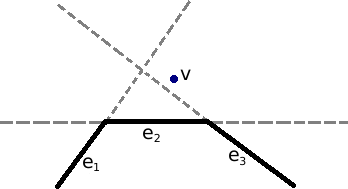
\includegraphics[width=0.5\textwidth]{three_edges.png}  \end{center}
Conceptually, we understand that $v$ should be allowed to cross the half spaces created by the edge segments, but not all three at once.  Further, if a corrective force (or impulse) is applied, then it should only be applied in the direction of a single edge's normal to prevent penetration on that edge.

First, collision detection would return the gap distance for $v$ in each of the half spaces.  Let these values be $\psi_1$, $\psi_2$, and $\psi_3$.  Observing the figure above, we notice that $\psi_1$ is negative, while $\psi_2$ and $\psi_3$ are positive.   

We proceed by defining the following variables: 
\begin{center}
$c_2 = max(0, \psi_1 - \psi_2)  $ \\
$c_3 = max(0, \psi_1 - \psi_3)  $ 
\end{center}
We then write the non-penetration constraints as follows: 

\[ 
\begin{matrix}
0 \leq & c_2 - \psi_2 + \psi_1 & \perp & c_2 & \geq 0 \\
0 \leq & c_3 - \psi_3 + c_2 + \psi_1 & \perp & c_3 & \geq 0 \\
\end{matrix}
\]
\[
\begin{matrix}  
0 \leq & d_1 + \psi_1 & \perp & d_1 & \geq 0 \\
0 \leq & d_2 + \psi_2 & \perp & d_2 & \geq 0 \\
0 \leq & d_3 + \psi_3 & \perp & d_3 & \geq 0 
\end{matrix} 
\]
\[
\begin{matrix}  
0 \leq & d_1 + (c_2 + c_3) + \psi_1 & \perp & \lambda_1 & \geq 0 \\
0 \leq & d_2 + (c_2 + c_3) + \psi_2 & \perp & \lambda_2 & \geq 0 \\
0 \leq & d_3 + (c_2 + c_3) + \psi_3 & \perp & \lambda_3 & \geq 0 \\
\end{matrix} 
\]
\[
(c_2 + c_3) + \psi_1 \geq 0
\]

Let's take a close look at the first two lines of constraints.  

\newpage
Searching for the general formulation with $m$ facets...  \\
$Lemma$ 4.2.1: $max(a,0) \iff 0 \leq b-a \perp b \geq 0$ \\
$Lemma$ 4.2.2: $b = |min(a,0)| \iff 0 \leq b + a \perp b \geq 0$ \\
\line(1,0){300} \\  \textbf{2 Facets} 

We want to ensure that $max(\psi_1,\psi_2) \geq 0$:  \\ \\
$max(\psi_1, \psi_2) = \psi_2 + max(0, \psi_1 - \psi_2)$ \hspace{6mm}(4.4)  \\
Let $c_2 = max(0,\psi_1 - \psi_2)$ \hspace{2.4cm}(4.5) \\
$0 \leq c_2 - (\psi_1 - \psi_2) \perp c_2 \geq 0$ \hspace{2cm}(4.6) \\  \\
$0 \leq max(\psi_1, \psi_2) \perp \lambda_j \geq 0 $ \\
Plugging in 4.4 and using 4.5: \\
$0 \leq c_2 + \psi_2 \perp \lambda_1 \geq 0$ \hspace{3cm}(4.7) \\
$0 \leq c_2 + \psi_2 \perp \lambda_2 \geq 0$  \hspace{3cm}(4.8) \\ \\
We can follow the same procedure using the same lemmas for more edges: \\ 
\line(1,0){300} \\  \textbf{3 Facets} \\
$max(\psi_1,\psi_2, \psi_3) = max(max(\psi_1,\psi_2),\psi_3)$ \\
$= max(\psi_2 + max(0,\psi_1-\psi_2), \psi_3)$  \\
$= \psi_3 + max(0, \psi_2 + max(0,\psi_1-\psi_2) - \psi_3)$  \hspace{10mm} (Similar to 4.4) \\
Let $c_3 = max(0,\psi_2 + max(0, \psi_1 - \psi_2) - \psi_3)$\hspace{9mm} (Similar to 4.5)  \\
$0 \leq c_3 - [\psi_2 + max(0, \psi_1 - \psi_2) - \psi_3] \perp c_3 \geq 0$  \hspace{5mm} (Similar to 4.6) \\ \\
$0 \leq max(\psi_1, \psi_2, \psi_3) \perp \lambda_j \geq 0$ \\
$0 \leq \psi_3 + c_3 \perp \lambda_1 \geq 0$ \\
$0 \leq \psi_3 + c_3 \perp \lambda_2 \geq 0$ \\
$0 \leq \psi_3 + c_3 \perp \lambda_3 \geq 0$ \\
\line(1,0){300} \\  \textbf{4 Facets} \\
$max(\psi_1,\psi_2,\psi_3, \psi_4) = max(max(\psi_1,\psi_2,\psi_3), \psi_4)$ \\
$= max(\psi_3 + max(0, \psi_2 + max(0,\psi_1 - \psi_2)-\psi_3), \psi_4)$  \\
$= \psi_4 + max(0, [\psi_3 + max(0, \psi_2 + max(0,\psi_1 - \psi_2)-\psi_3)]- \psi_4)$ \\
Let $c_4 = max(0, [\psi_3 + max(0,\psi_2 + max(0,\psi_1 - \psi_2)-\psi_3)]-\psi_4)$  \\
$0 \leq c_4 - [(\psi_3 + max(0, \psi_2 + max(0,\psi_1-\psi_2)-\psi_3)) -\psi_4] \perp c_4 \geq 0 $ \\ \\
$0 \leq max(\psi_1,\psi_2,\psi_3,\psi_4) \perp \lambda_j \geq 0 $ \\
$0 \leq \psi_4 + c_4 \perp \lambda_1 \geq 0$ \\
$0 \leq \psi_4 + c_4 \perp \lambda_2 \geq 0$ \\
$0 \leq \psi_4 + c_4 \perp \lambda_3 \geq 0$ \\
$0 \leq \psi_4 + c_4 \perp \lambda_4 \geq 0$ \\

Note the reccurence above of $c_2$ in $c_3$, as well as $c_3$ in $c_4$.
\newpage  
\line(1,0){300} \\ \textbf{m Facets} \\
$max(\psi_1,\psi_2,...,\psi_m) = max(max(\psi_1,...,\psi_{m-1}),\psi_m)$ \\
$= \psi_m + max(0,(\psi_{m-1}+ max(0,\psi_{m-2} + max( ... )-\psi_{m-1}))-\psi_m)$ \\
$= \psi_m + c_m$ \\ Then
\begin{center}
$ 0 \leq c_m - (\psi_{m-1} + c_{m-1} - \psi_m) \perp c_m \geq 0 $ 
\end{center}
where 
\begin{center}
$ c_2= max(0,\psi_1-\psi_2)$ \\ $c_i = max(\psi_{i-1} + c_{i-1}, \psi_i), $ for $i=3,...,m $
\end{center}

I think this means that the general formulation (with $c_i$ as defined) is slightly different than in Binh's thesis.  It should look more like (which is to say, this is not 100\% correct yet): 
\begin{center}
\line(1,0){300}  \\
$ 0 \leq c_2 - \psi_1 + \psi_2 \perp c_2 \geq 0 $ \\
$ 0 \leq c_3 - \psi_2 - c_2 + \psi_3 \perp c_3 \geq 0 $ \\
$ 0 \leq c_4 - \psi_3 - c_3 + \psi_4 \perp c_4 \geq 0 $ \\ 
$\vdots$ \\
$ 0 \leq c_m - \psi_{m-1} - c_{m-1} + \psi_m \perp c_m \geq 0 $ \\ \vspace{8mm}
$ 0 \leq d_1 + \psi_1 \perp d_1 \geq 0 $ \\
$ 0 \leq d_2 + \psi_2 \perp d_2 \geq 0 $ \\
$\vdots$ \\
$ 0 \leq d_m + \psi_m \perp d_m \geq 0 $ \\ \vspace{8mm}
$ 0 \leq d_1 + 0 + \psi_1 \perp \lambda_1 \geq 0 $  \\
$ 0 \leq d_2 + c_2 + \psi_2 \perp \lambda_2 \geq 0 $ \\
$\vdots$ \\
$ 0 \leq d_m + c_m + \psi_m \perp \lambda_m \geq 0 $ \\ \vspace{8mm}
$ c_m \geq 0 $ \\
\line(1,0){300}  
\end{center}

%%%%%%%%%%%%%%%%%%%%%%%%%%%%%%%%%%%%%%%%%%%%%%%%
%% August 1, 2012
%% I think we made progress understanding the MCP formulation of CDA today.
%% 
\newpage
\section{CDA in 3D}
Before we formulate the constraints and dynamics, let us define several terms.  Consider the 2D case of body $B_1$ near body $B_2$ and the possible vertex-edge collisions.  There are 3 \emph{contacts} with 7 total possible \emph{subcontacts}: $v_1$ with edges $(e_3, e_4, e_5)$, $v_2$ with edges $(e_1, e_2)$, or $v_3$ with edges ($e_1$, $e_2$).  Let contact $C_1$ include vertex $v_1$, then we say that vertex $v_1$ is in contact with the \emph{mainfold} consisting of $(e_3, e_4, e_5)$.  It is possible for a manifold to contain zero or all of the edges of a body; this is determined by the collision detection routine.  \\ \\
Number of contacts: $n_c$  \\
Number of subcontacts (facets) in a given manifold: $n_s$  \\
Number of friction directions: $n_d$  \\
Time step size: $h$ 
\subsection{MCP Formulation}
\begin{equation}
\begin{vmatrix}
0 \\ \rho_{n}^{l+1} \\ \rho_{f}^{l+1} \\ c_{a}^{l+1}  \\ \sigma^{l+1} 
\end{vmatrix} =
\begin{vmatrix} 
M & -G_{n} & -G_{f} & 0 & 0 \\
G_{n}^{T} & 0 & 0 & E_1 & 0 \\
G_{f}^{T} & 0 & 0 & 0 & E \\
G_a^{T} & 0 & 0 & E_2 & 0 \\
0 & U & -E^{T} & 0 & 0 
 \end{vmatrix} 
\begin{vmatrix}
\nu^{l+1} \\
p_{n}^{l+1} \\
p_{f}^{l+1} \\
c_{a}^{l+1} \\
s^{l+1}
\end{vmatrix} + 
\begin{vmatrix}
-M\nu^{l}-p_{ext}^{l} \\
\Psi_{n}^{l}/h \\
0 \\
\Delta \Psi_a / h  \\
0
\end{vmatrix}
\end{equation}


where each of the submatrices are defined in terms of the bodies found to be in contact, indexed over $n_c$ contacts by the $i^{th}$ body and $j^{th}$ contact, i.e.\\
\begin{equation}
M = blockdiag(M_1,...,M_{n_c})
\text{ where } 
M_i = \begin{bmatrix} m_iI_{(3\times3)} & \mathbf{0} \\ \mathbf{0} & J_{i (3\times3)}  \end{bmatrix}, 
\nonumber
\end{equation}


\begin{equation}
G_{n_{ij}} = \begin{bmatrix} 
\hat{n}_{ij}  \\ 
(r_{ij} \times \hat{n}_{ij})_{Z}
\end{bmatrix},  \nonumber
\end{equation}

\begin{equation}
G_{f_{ij}} = \begin{bmatrix} 
\hat{d}_{ij1} & ... & \hat{d}_{ijn_d} \\
(r_{ij} \times  \hat{d}_{ij1})_Z  & ... & (r_{ij} \times  \hat{d}_{ijn_d})_Z
\end{bmatrix}, 
\nonumber
 \end{equation}

\begin{equation}
 G_{a}^T = \begin{bmatrix} G_{a_1}^T \\  \vdots  \\  G_{a_{n_c}}^T\end{bmatrix}  \nonumber
\text{ where }
 G_{a_j}^T = \begin{bmatrix} G_{n_1}^T - G_{n_2}^T \\  \vdots  \\  G_{n_1}^T  -  G_{n_s}^T \end{bmatrix},
\nonumber
\end{equation}

\begin{equation}
 \Psi_a = \begin{bmatrix} \Psi_{a_1} \\ \vdots \\ \Psi_{a_{n_s}} \end{bmatrix} \text{ where }
 \Psi_{a_j} = \begin{bmatrix} \Psi_1 - \Psi_2 \\ \vdots  \\ \Psi_1 - \Psi_{n_s} \end{bmatrix}, 
\nonumber
\end{equation}

\begin{equation}
U = diag(\mu_{1}, \hspace{2mm} \ldots \hspace{2mm}, \mu_{n_s}  ),  \nonumber
 \end{equation}

\begin{equation}
E = blockdiag
    \begin{pmatrix}
	\begin{vmatrix} 1 \\ 1 \\ \vdots \end{vmatrix}_1 , \hspace{2mm} \ldots \hspace{2mm} , 
	\begin{vmatrix} 1 \\ 1 \\ \vdots \end{vmatrix}_{n_c}  \nonumber 
    \end{pmatrix}
\end{equation}
where each column vector of ones has length equal to the number of friction directions in the friction cone.

\begin{equation}
E_1 = blockdiag(E_{1_1}, \dots , E_{1_{n_c}}) \text{ where } E_{1_j} = ones(n_s - n_d,1) \text{(is this true?)}
\nonumber
\end{equation}

\begin{equation}
E_2 = blockdiag(E_{2_1}, \dots , E_{2_{n_c}}) \text{ where } E_{2_j} = tril(ones(n_s - 1))
\nonumber
\end{equation}

After the MCP is formed using the information from the collision detection routine, it is passed to the PATH solver [4].  

\paragraph{State Updates}
For each body $P_{i}$ involved in a collision, $\nu_{i}^{l+1}$ is extracted from a solution of the MCP and used to update the body, 
\begin{center}
$
\nu_{i} \gets \nu_{i}^{l+1}    \nonumber
$ 

$
u_{i} \gets u_{i} + h \nu_{i}^{l+1}   \nonumber
$. 
\end{center}
For bodies not in contact, 
\begin{center}
$
\nu_{i} \gets \nu_{i} + h \frac{F_{ext_i}}{m_{i}}
$

$
u_{i} \gets u_{i} + h \nu_{i}
$.
\end{center}


\end{document} 


































